% JAC-ECC 2026 IEEE Conference Paper Draft (DOUBLE-BLIND SUBMISSION)
% Neuro-Symbolic Breast Cancer Diagnosis Using DeepProbLog and Medical Knowledge
%
% Compile with: pdflatex main && bibtex main && pdflatex main && pdflatex main
%
% CAMERA-READY: After acceptance, restore the real author block below and
% re-add acknowledgments/funding if desired. Do not include those in review.
%
\documentclass[conference]{IEEEtran}

\usepackage{amsmath,amssymb,amsfonts}
\usepackage{graphicx}
\usepackage{cite}
\usepackage{booktabs}
\usepackage{url}
\usepackage{xcolor}
\usepackage{listings}
\renewcommand{\ttdefault}{cmtt}
\usepackage{tikz}
\lstset{
  basicstyle=\ttfamily\scriptsize,
  breaklines=true,
  columns=fullflexible,
  keepspaces=true,
  frame=none,
  aboveskip=4pt,
  belowskip=4pt,
  xleftmargin=0pt
}
\usetikzlibrary{arrows.meta,positioning,fit,calc}

% Revision colour: change blue to black for the final submission.
\colorlet{revcolor}{blue}
\newcommand{\rev}[1]{\textcolor{revcolor}{#1}}
\newenvironment{revblock}{\color{revcolor}}{}

% Optional: uncomment for draft notes visibility
% \newcommand{\todo}[1]{\textcolor{red}{\textbf{[TODO: #1]}}}
\newcommand{\todo}[1]{\textit{[TODO: #1]}}

% Clear identifying PDF metadata for double-blind review.
\pdfinfo{
  /Title (Neuro-Symbolic Breast Cancer Diagnosis Using DeepProbLog and Medical Knowledge)
  /Author ()
  /Subject ()
  /Keywords ()
  /Creator (LaTeX with IEEEtran)
  /Producer ()
}

\begin{document}

\title{Neuro-Symbolic Breast Cancer Diagnosis Using DeepProbLog and Medical Knowledge}

% -------------------------------------------------------------------------
% JAC-ECC 2026 double-blind: no names, affiliations, emails, or acknowledgments.
% Restore the camera-ready author block after acceptance (kept commented below).
% -------------------------------------------------------------------------
% \author{\IEEEauthorblockN{Anonymous Author(s)}
% \IEEEauthorblockA{Affiliation withheld for double-blind review}}

% CAMERA-READY AUTHOR BLOCK (do not use for review submission):
% \author{\IEEEauthorblockN{Author Name}
% \IEEEauthorblockA{Affiliation\\
% City, Country\\
% Email: author@institution.edu}}

\maketitle

\begin{abstract}
End-to-end networks for breast cancer diagnosis usually return only a malignancy score. This paper uses DeepProbLog for explainability so that the obtained score is computed from named findings. A residual network with 18 layers (ResNet18), pretrained on ImageNet, shares one trunk among four heads that estimate lesion kind, mass shape, mass margin, and calcification type. Those terms come from the Breast Imaging Reporting and Data System (BI-RADS) lexicon. A short probabilistic program turns the uncertain findings into a malignancy probability and a trace of which rule fired. The images are lesion crops from the Curated Breast Imaging Subset of the Digital Database for Screening Mammography (CBIS-DDSM). On the test images, the area under the receiver operating characteristic curve of the proposed DeepProbLog architecture is $0.752$, against $0.746$ for a baseline ResNet18 that predicts malignancy directly. \rev{This difference is not statistically significant (paired DeLong test, $p=0.79$), so the contribution is the decision trace rather than a gain in accuracy. Applied to the recorded findings, the three rules reach a sensitivity of $0.805$, which shows how much of the error comes from the rules and how much from the heads. Knowing the evidence behind the network decision is valuable for the treating physician and for explainable AI.}
\end{abstract}

\begin{IEEEkeywords}
Breast cancer diagnosis, neuro-symbolic AI, DeepProbLog, probabilistic logic programming, medical image analysis, explainable AI, BI-RADS
\end{IEEEkeywords}

\section{Introduction}
\label{sec:introduction}

Breast cancer is among the most commonly diagnosed cancers worldwide and a major cause of cancer-related mortality in women~\cite{sung2021global}. Mammography is a primary screening examination. Deep networks now classify breast images with high accuracy, but the usual output is a single malignancy score~\cite{litjens2017survey,balkenende2022application}. In a high-stakes setting, a score without the finding that produced it is difficult to check~\cite{rudin2019stop,vandervelden2022xai}.

One alternative is to predict clinically named visual concepts and then apply explicit domain knowledge~\cite{koh2020concept}. DeepProbLog supports that split: neural predicates supply probabilities, and a probabilistic logic program combines them~\cite{manhaeve2018deepproblog,manhaeve2021neural}. This paper uses that split for mammography. Four heads on one ResNet18 trunk extracts lesion and calcification types, mass shape and mass margin (using terminology from the Breast Imaging Reporting and Data System (BI-RADS) lexicon~\cite{acr2013birads}). A three-rule program turns those probabilities into $P(\mathrm{malignant})$ and names the rule that fired. A baseline ResNet18 that maps the image directly to malignancy/ non-malignancy binary decision is used for \rev{comparison}.

This paper is organized as follows. Section~\ref{sec:related} reviews related work. Section~\ref{sec:methodology} describes the model and the program. Section~\ref{sec:experiments} describes the data and the training setup. Section~\ref{sec:results} reports the results \rev{with confidence intervals, measures the ceiling of the rules on the recorded findings,} and walks through one decision trace. Section~\ref{sec:conclusion} concludes the paper.

\section{Related Work}
\label{sec:related}

\subsection{Deep Learning for Breast Cancer Image Classification}
Deep learning is widely used in medical image analysis, including mammography classification and computer-aided diagnosis. Residual networks are common pretrained feature extractors~\cite{he2016resnet}. Public collections include the Curated Breast Imaging Subset of the Digital Database for Screening Mammography (CBIS-DDSM)~\cite{lee2017cbis} and Breast Ultrasound Images (BUSI)~\cite{aldhabyani2020busi}. This study uses CBIS-DDSM mammograms only. Many published systems predict the label from the image directly and do not expose a concept layer that a symbolic program can read.

\subsection{Explainable Models in Medical Imaging}
Clinical use needs an explanation that can be checked, not only a single score~\cite{vandervelden2022xai,rudin2019stop}. Post-hoc methods explain a trained black box after the decision.  Other models extract the evidences first, then decide the diagnosis from them~\cite{koh2020concept}. This paper keeps the concept layer (evidence), but the step from concepts to malignancy is a probabilistic logic program rather than a second neural network.

\subsection{Neuro-Symbolic Reasoning}
Neuro-symbolic models combine neural perception with symbolic rules~\cite{garcez2002neural,garcez2023neurosymbolic}. ProbLog attaches probabilities to logical facts~\cite{deraedt2007problog}. DeepProbLog lets a neural network supply those probabilities, then runs the usual probabilistic inference~\cite{manhaeve2018deepproblog,manhaeve2021neural}. The program in this paper describes this inference step: it does not replace the rules with an equivalent set of ordinary conditionals hidden inside another network.

\section{Proposed Neuro-Symbolic Approach}
\label{sec:methodology}

A mammogram image crop is read by one network with four heads. DeepProbLog treats each head as a neural predicate and applies the program given below. The output is $P(\mathrm{malignant})$ together with the rule that contributed most to that probability. Figure~\ref{fig:architecture} shows the proposed architecture.

\subsection{Overall Architecture}
\label{sec:architecture}

The shared trunk feeds four heads. Each head is passed to DeepProbLog as an uncertain fact, and the rules produce the score and the trace.

\begin{figure}[!t]
\centering
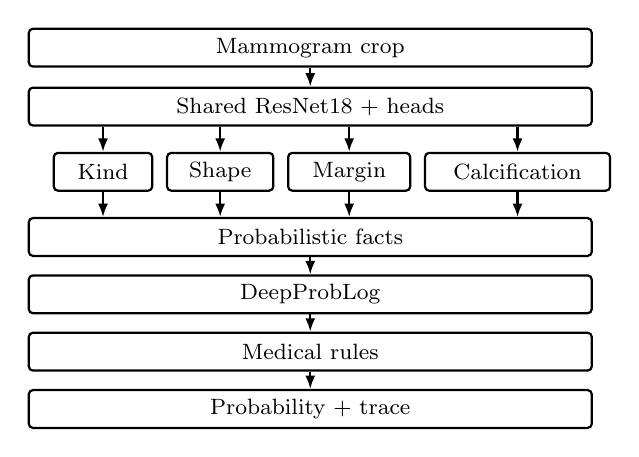
\begin{tikzpicture}[
  font=\footnotesize,
  box/.style={
    draw,
    rounded corners=1.5pt,
    align=center,
    inner sep=2.5pt,
    minimum height=0.48cm,
    thick
  },
  wide/.style={box, minimum width=7.15cm},
  arr/.style={
    -{Latex[length=1.7mm]},
    thick
  }
]
  \node[box, minimum width=1.25cm] (kind) {Kind};
  \node[box, minimum width=1.35cm, right=0.16cm of kind] (shape) {Shape};
  \node[box, minimum width=1.55cm, right=0.16cm of shape] (margin) {Margin};
  \node[box, minimum width=2.35cm, right=0.16cm of margin] (calc) {Calcification};

  \coordinate (headtop) at ($(kind.north)!0.5!(calc.north)$);
  \coordinate (headbot) at ($(kind.south)!0.5!(calc.south)$);
  \node[wide, anchor=south] (nn) at ([yshift=0.32cm]headtop) {Shared ResNet18 + heads};
  \node[wide, anchor=south] (mammo) at ([yshift=0.24cm]nn.north) {Mammogram crop};
  \node[wide, anchor=north] (facts) at ([yshift=-0.32cm]headbot) {Probabilistic facts};
  \node[wide, below=0.22cm of facts] (dpl) {DeepProbLog};
  \node[wide, below=0.22cm of dpl] (rules) {Medical rules};
  \node[wide, below=0.22cm of rules] (out) {Probability + trace};

  \draw[arr] (mammo) -- (nn);
  \draw[arr] (nn.south -| kind.north) -- (kind.north);
  \draw[arr] (nn.south -| shape.north) -- (shape.north);
  \draw[arr] (nn.south -| margin.north) -- (margin.north);
  \draw[arr] (nn.south -| calc.north) -- (calc.north);
  \draw[arr] (kind.south) -- (kind.south |- facts.north);
  \draw[arr] (shape.south) -- (shape.south |- facts.north);
  \draw[arr] (margin.south) -- (margin.south |- facts.north);
  \draw[arr] (calc.south) -- (calc.south |- facts.north);
  \draw[arr] (facts) -- (dpl);
  \draw[arr] (dpl) -- (rules);
  \draw[arr] (rules) -- (out);
\end{tikzpicture}
\caption{The proposed architecture: an image crop is read by a shared trunk with four heads. DeepProbLog applies the rules and returns a malignancy probability and a trace.}
\label{fig:architecture}
\end{figure}

\subsection{What the Four Heads Predict}
\label{sec:concepts}

The trunk is an ImageNet-pretrained residual network with 18 layers (ResNet18)~\cite{he2016resnet}. After pooling it yields a 512 features-vector, that is read by each of the four heads. Each head ends with a softmax activation function. The four heads together produce twelve probabilities. Table~\ref{tab:heads} lists the classes.

\begin{table}[!t]
\caption{Classes predicted by the four heads.}
\label{tab:heads}
\centering
\footnotesize
\begin{tabular}{@{}l p{3.55cm}@{}}
\toprule
Head & Classes \\
\midrule
Lesion kind & mass, calcification \\
Mass shape & regular, irregular, unknown \\
Mass margin & circumscribed, spiculated, other, unknown \\
Calcification type & absent, typically benign, suspicious \\
\bottomrule
\end{tabular}
\end{table}

The class names follow the BI-RADS lexicon~\cite{acr2013birads,lee2017cbis}. Lesion kind is the abnormality itself: a mass or a calcification. Mass shape has three groups. Round, oval, and lobulated shapes are recorded as regular. Irregular shape and architectural distortion are recorded as irregular. Otherwise, the shape is considered as unknown. \rev{Mass margin has four classes (Table~\ref{tab:heads}). A margin that includes spiculated is recorded as spiculated, otherwise a circumscribed margin is recorded as circumscribed. Indistinct (written ILL\_DEFINED in CBIS-DDSM), microlobulated, and obscured margins are grouped as other, and a missing margin is unknown.} Calcification has three groups. Pleomorphic, amorphous, and fine-linear or branching morphologies are recorded as suspicious. Every other calcification morphology\rev{, including a missing one,} is typically benign. If lesion kind is of type mass, calcification type is marked absent.

\subsection{The Implemented DeepProblog Program}
\label{sec:knowledge}
\label{sec:problog}
The DeepProbLog program listed below describes only the first part of the fifth edition of BI-RADS which focuses on what is visible in the mammogram. It identifies irregular shapes, spiculated margins, and suspicious calcification morphology as the primary indicators of malignancy. \rev{It is a small working subset of the lexicon, not the full BI-RADS assessment: indistinct and microlobulated margins and calcification distribution are not antecedents of the trained rules. Section~\ref{sec:whysmall} gives the reason.}
\begin{lstlisting}
nn(kind_net, [X], Y, [mass, calcification])
    :: lesion_kind(X, Y).
nn(shape_net, [X], Y,
    [regular, irregular, unknown])
    :: shape(X, Y).
nn(margin_net, [X], Y, [circumscribed,
    spiculated, other, unknown])
    :: margin(X, Y).
nn(calc_net, [X], Y, [absent,
    typically_benign, suspicious])
    :: calc(X, Y).

malignant(X) :- lesion_kind(X, mass),
    shape(X, irregular).
malignant(X) :- lesion_kind(X, mass),
    margin(X, spiculated).
malignant(X) :- lesion_kind(X, calcification),
    calc(X, suspicious).
\end{lstlisting}
 Each \texttt{nn} line -in the above program- binds one head to a predicate. Consider the first predicate "kind net" which corresponds to the "lesion kind" head, "X" is the input image, 
"Y" is the output result  and
"mass, calcification" is the list of allowed values for "Y". The same pattern governs the other three heads. 
The above program also include three rules that determine the type of the malignancy found in the input image. For example, the first rule says that an image "X" is classified as malignant if the  lesion kind is "mass" and its shape is "irregular". A rule succeeds and contributes a  probability only when both of its conditions hold.


\subsection{Inference in DeepProbLog}
\label{sec:inference}

DeepProbLog program is given a query \texttt{malignant(X)}. It computes its success probability from the four heads~\cite{manhaeve2021neural}. \rev{This is the probability that at least one rule is provable, computed exactly by knowledge compilation, as in standard ProbLog semantics. It is not the largest rule product. Each head is a neural annotated disjunction, so its classes are mutually exclusive, and the four heads are treated as independent given the image. Rules~1 and~2 share the fact \texttt{lesion\_kind(X, mass)}, and mass and calcification exclude each other, so}
\begin{revblock}
\begin{multline}
P(\mathrm{malignant}) = P(\mathrm{mass})\,\big[P(\mathrm{irr}) + (1-P(\mathrm{irr}))\,P(\mathrm{spic})\big] \\
+ P(\mathrm{calc})\,P(\mathrm{susp}),
\label{eq:query}
\end{multline}
\end{revblock}
\rev{where irr, spic, calc, and susp denote irregular shape, spiculated margin, lesion kind calcification, and suspicious calcification. Within the mass branch, rules~1 and~2 combine as a noisy-OR. The same query probability is used in training, in the threshold, and in every reported metric. For the trace only, the rule whose body has the largest probability is reported as the rule that fired. It explains the score and does not change it.}


\section{Experimental Setup}
\label{sec:experiments}

\subsection{Dataset and Images}
\label{sec:dataset}

The images come from CBIS-DDSM~\cite{lee2017cbis}, a curated subset of the Digital Database for Screening Mammography. The images are digitized screen-film mammograms. For each annotated abnormality the release contains three pictures: the full breast image, a crop centered on the lesion, and a binary mask of that lesion. We use only the grayscale crop. The shape, margin, and calcification descriptors refer to the abnormality. Mass crops and calcification crops are pooled into one set of abnormalities.

Table II, shows how the dataset has been split into training (69\%), validation (\rev{12.9\%}) and testing (18\%). Care has been taken so that no patient appears in more than one split. \rev{After the mass and calcification files are merged, the official CBIS-DDSM split places 31 patients in both training and test. All their rows were moved to training, so the test set keeps 644 of the official 704 images, and the validation set is drawn from the training patients with a grouped split (seed 42). The numbers are therefore not directly comparable with work that reports results on the official split.} The recorded pathology has three values: malignant, benign, and benign without callback. Benign without callback means a benign finding for which no further recall has been indicated. Both non-malignant values are treated as the negative class. They are not clinically the same; the merge only defines the binary task. 



\begin{table}[!t]
\caption{Cropped images in each split, before augmentation.}
\label{tab:dataset}
\centering
\footnotesize
\setlength{\tabcolsep}{3.5pt}
\begin{tabular}{@{}lrrr@{}}
\toprule
Split & Images & Patients & Malignant \\
\midrule
Train & 2462 (69.0\%) & 1060 (67.7\%) & 1019 (41.4\%) \\
Validation & 462 (12.9\%) & 188 (12.0\%) & 181 (39.2\%) \\
Test & 644 (18.0\%) & 318 (20.3\%) & 257 (39.9\%) \\
\bottomrule
\end{tabular}

\vspace{0.4em}
\begin{minipage}{\columnwidth}
\footnotesize
Image and patient percentages are shares of 3568 images and 1566 patients. The malignant percentage is the share of the original images in that split, before augmentation.
\end{minipage}
\end{table}

\begin{table}[!t]
\caption{Copies added to the training split so both classes have the same number of images.}
\label{tab:augmentation}
\centering
\footnotesize
\begin{tabular}{@{}lrr@{}}
\toprule
Class & Copies added & After \\
\midrule
Benign & 2886 & 4329 (50\%) \\
Malignant & 3310 & 4329 (50\%) \\
\midrule
Total & 6196 & 8658 \\
\bottomrule
\end{tabular}

\vspace{0.4em}
\begin{minipage}{\columnwidth}
\footnotesize
The percentage is the share of the 8658 training images after augmentation.
\end{minipage}
\end{table}

\subsection{\rev{Why the Input Size Is 224 $\times$ 224 Pixels}}
\label{sec:resolution}

The downloaded 3568 crops do not share the same size. Every crop is adjusted to $224\times 224$ pixels, which corresponds to 70\% to 100\% of the original crop. This choice has been made due to our hardware platform limitations. Crops smaller than 224 x 224 pixels are enlarged, which blurs the margin. Crops much larger than 224 x 224  pixels are reduced. Because 41.4\% of training abnormalities are malignant, extra training copies are added until each class has 4329 images. Data augmentation has been done by horizontal flipping, rotation by up to 12 degrees, or mild shifting and rescaling.


\subsection{Training}
\label{sec:neural}

The training has two stages. Both run on two NVIDIA T4 graphics processing units (on Kaggle).

\rev{\textit{Stage 1, without DeepProbLog.}} The proposed architecture is trained in supervised mode. The four heads are trained for eight epochs to match the recorded findings, at a learning rate of $3\times10^{-4}$. In the first two epochs, the trunk is frozen, so only the heads learn. In the next six epochs, the trunk learns as well, at a learning rate of $3\times10^{-5}$, which is one tenth of the heads learning rate. \rev{Only the concept labels are used, with batch size 16. With $\hat{y}_h$ the softmax output of head $h$ and $c_h$ the recorded class, the loss is}
\begin{revblock}
\begin{equation}
\mathcal{L}_1 = \sum_{h \in \{\mathrm{kind},\,\mathrm{shape},\,\mathrm{margin},\,\mathrm{calc}\}} -\,w_{h,c_h} \log \hat{y}_h(c_h),
\label{eq:stage1}
\end{equation}
\end{revblock}
\rev{where $w_{h,c}$ is an inverse-frequency class weight computed on the training images before augmentation.}

\rev{\textit{Stage 2, with DeepProbLog.}} The same architecture is then trained for 15 more epochs, at a learning rate of $3\times10^{-4}$ and batch size 2. The trunk remains trainable at the lower learning rate of $3\times10^{-5}$. \rev{Both the malignancy label and the concept labels are used. Each training image $x$ gives five queries: \texttt{malignant(x)} with target $t=1$ for malignant and $t=0$ otherwise, whose probability is Eq.~(\ref{eq:query}), and one query per head for its recorded class, \texttt{lesion\_kind(x,$c_\mathrm{kind}$)}, \texttt{shape(x,$c_\mathrm{shape}$)}, \texttt{margin(x,$c_\mathrm{margin}$)}, and \texttt{calc(x,$c_\mathrm{calc}$)}, each with target $t=1$. For a batch $B$ of queries with probabilities $p_q$,}
\begin{revblock}
\begin{equation}
\mathcal{L}_2 = -\frac{1}{|B|}\sum_{q \in B} \big[t_q \log p_q + (1-t_q)\log(1-p_q)\big].
\label{eq:stage2}
\end{equation}
\end{revblock}
\rev{All five queries have equal weight. The gradient of the malignancy query passes through Eq.~(\ref{eq:query}) to the four heads and the trunk, so the program is part of the training.}

The baseline is a ResNet18 with a single two-class output, malignant or not. It is trained for 15 epochs on the same images and the same splits, with no logic program. \rev{The comparison is not budget-matched: the proposed model trains for $8+15$ epochs and uses four extra concept labels, while the baseline trains for 15 epochs on the malignancy label only.}

\subsection{Performance Metrics}
\label{sec:metrics}

We adopted the accuracy, sensitivity, specificity, and the area under the receiver operating characteristic curve (ROC-AUC), as our performance metrics. Accuracy is the proportion of correct predictions (both positive and negative) out of the total number of predictions. Sensitivity is the share of malignant cases that are caught. Specificity is the share of non-malignant cases that are correctly predicted as negative. \rev{Macro-F1 is the unweighted mean of the F1 scores of the two classes. The 95\% confidence interval of each ROC-AUC comes from 2000 paired bootstrap resamples of the test images, and the two ROC-AUCs are compared with the paired DeLong test~\cite{delong1988comparing}.}

\section{Results and Discussion}
\label{sec:results}
\rev{The operating point} is affected by a good choice of the cutoff threshold on $P(\mathrm{malignant})$. A case with $P(\mathrm{malignant})$ $\geq$ cutoff is considered malignant otherwise it is considered benign. The threshold is chosen on the validation images only\rev{, from 0.05 to 0.95 in steps of 0.01, and is kept unchanged for the test images. Changing the threshold does not change the trained model; it only moves its operating point between sensitivity and specificity.} Table~\ref{tab:comparison} shows the effect of \rev{the threshold rule} on the test performance. \rev{A designer should select the operating point that matches the clinical goal.} For breast cancer diagnosis one should target the sensitivity metric since it avoids missing a positive case.



Table~\ref{tab:comparison} compares the selected model (first row in Table~\ref{tab:comparison}) with the base model on the 644 test abnormalities. The ROC-AUC values are $0.752$ for DeepProbLog and $0.746$ for the baseline. \rev{The 95\% bootstrap intervals are $[0.712, 0.789]$ and $[0.707, 0.784]$. The paired DeLong test gives a difference of $0.005$, with a 95\% interval of $[-0.035, 0.046]$ and $p=0.79$, so the two models rank the test cases equally well. These results come from a single training run.} \rev{\todo{add the extra-seed results when the seed 7 run finishes}} \rev{On validation, the recorded class receives a probability of at least 0.5 for} 90.5\% \rev{of the images for} the lesion kind head, 72.3\% \rev{for} the shape head, 70.1\% \rev{for} the margin head, and 82.0\% \rev{for} the calcification head. Sensitivity and specificity differ because each row uses a different threshold. The lower specificity of the selected model is the cost of the higher sensitivity. \rev{Within the swept range, no baseline threshold reaches a validation sensitivity of 0.80. A lower threshold would reach it: on the test ROC curve, the baseline needs a threshold of 0.022 to reach a sensitivity of 0.80, where its specificity is 0.540, against 0.556 for DeepProbLog at the same sensitivity. At matched sensitivity the two models are therefore close.}

\begin{table}[!t]
\caption{Test comparison on 644 images.}
\label{tab:comparison}
\centering
\footnotesize
\setlength{\tabcolsep}{4pt}
\begin{tabular}{@{}lcccccc@{}}
\toprule
Model & Valid Thr. & Acc. & Sens. & Spec. & Macro-F1 & AUC \\
\midrule
DeepProbLog & 0.55$^{*}$ & 0.654 & \textbf{0.798} & 0.558 & 0.654 & \textbf{0.752} \\
DeepProbLog & 0.60$^{\dagger}$ & 0.666 & 0.716 & 0.633 & 0.663 & \textbf{0.752} \\
ResNet18 & 0.50 & 0.689 & 0.591 & \textbf{0.755} & 0.674 & 0.746 \\
ResNet18 & 0.44$^{\ddagger}$ & \textbf{0.693} & 0.611 & 0.747 & \textbf{0.679} & 0.746 \\
\bottomrule
\end{tabular}

\vspace{0.45em}
\begin{minipage}{\columnwidth}
\footnotesize
$^{*}$\rev{Among validation thresholds with sensitivity at least 0.80, the one with the highest validation specificity.}\\
$^{\dagger}$Validation threshold with the highest macro-F1.\\
$^{\ddagger}$The baseline never reached sensitivity 0.80 on validation \rev{within the swept range}. This is the threshold that best balances its sensitivity and specificity.\\
\rev{AUC 95\% bootstrap CI: DeepProbLog $[0.712, 0.789]$, ResNet18 $[0.707, 0.784]$; DeLong $p=0.79$.}\\
Valid Thr.: validation threshold. Acc.: accuracy. Sens.: sensitivity. Spec.: specificity. AUC: area under the curve, which does not depend on a fixed threshold.
\end{minipage}
\end{table}



\subsection{\rev{Why the Gain Is Small}}
\label{sec:whysmall}

A gain of $0.006$ in ROC-AUC is not a large improvement\rev{, and the DeLong test shows it is not significant. At both thresholds the accuracy and macro-F1 of DeepProbLog are lower than those of the baseline.} Two limitations are behind this result:
\begin{itemize}
\item Both systems start from the same ResNet18  architecture pretrained on ImageNet. Next, they are  finetuned on the same $224\times224$ crops.

\item \rev{The three rules do not cover every malignant case. For example, patient P\_00017 has a malignant mass with a round shape, recorded as regular. Its margin is circumscribed in one view and ill-defined (indistinct) in the other, which falls into other. No rule matches either view even with correct concepts. This is a gap in the rules, not label noise: an indistinct margin is suspicious in BI-RADS.}

\end{itemize}

\begin{revblock}
\textit{Ceiling of the rules.} To separate the rules from the heads, the program was applied to the recorded concepts of the 644 test images, without the network (Table~\ref{tab:ceiling}). With these certain facts, the three rules reach a sensitivity of 0.805 and a specificity of 0.587. Extending the margin rules to indistinct and microlobulated margins, and treating a missing calcification type as unknown, raises the sensitivity to 0.918 but lowers the specificity to 0.468. ROC-AUC moves from 0.696 to 0.693, so the trained rules were left unchanged: the comparison is on ROC-AUC, and the extension does not improve it. Indistinct margins are suspicious in BI-RADS and common (24.5\% of training mass crops, 30.6\% of test mass crops); they stay in other because the added rule does not improve ranking. Microlobulated margins are uncommon (8.5\% and 6.4\%), so a separate trained class would be small, and the same check shows no ROC-AUC gain. The margin head was not retrained on these classes. That retraining, and calcification distribution, are left for future work.

\textit{Rules or heads.} At the 0.55 threshold, DeepProbLog makes 223 errors on the test images. In 130 of them (58\%; 21 missed malignancies and 109 false alarms), the rules give the wrong answer even on the recorded concepts, so the error comes from the rules. In the other 93 (42\%; 31 missed malignancies and 62 false alarms), the rules would give the correct answer on the recorded concepts, so the error comes from the heads.

\todo{Stage 1 alone vs.\ Stage 2 on the paper weights, and test accuracy and confusion matrices of the four heads (evaluation of the saved checkpoints on Kaggle)}
\end{revblock}

\begin{table}[!t]
\color{revcolor}
\caption{The three rules applied to the recorded concepts of the 644 test images (no network).}
\label{tab:ceiling}
\centering
\footnotesize
\setlength{\tabcolsep}{4pt}
\begin{tabular}{@{}lccccc@{}}
\toprule
Margin rules & Acc. & Sens. & Spec. & Macro-F1 & AUC \\
\midrule
Spiculated (as trained) & 0.674 & 0.805 & 0.587 & 0.674 & 0.696 \\
+ indistinct, microlobulated & 0.648 & 0.918 & 0.468 & 0.645 & 0.693 \\
\bottomrule
\end{tabular}
\end{table}


\subsection{A Decision Trace}
\label{sec:traces}

We consider the case of a benign mass (P\_00061) (whose ground truth description is: lesion kind= mass, shape= regular, margin = circumscribed, and calcification= absent) that has been misclassified by the model to highlight the practical utility of the decision trace. A standard black-box network would merely output a highly misleading malignancy score, leaving us with no clue to detect the error. Table~\ref{tab:trace}, gives the logic program findings with their corresponding probabilities. The root cause of this failure is that the neural head "lesion kind" misidentified the mass as a calcification (with a probability of 0.99\rev{),} which is multiplied by $P(\mathrm{calcification}=\mathrm{suspicious})=0.919$ \rev{in Eq.~(\ref{eq:query}) to yield $P(\mathrm{malignant})=0.91$. The mass branch adds almost nothing, because $P(\mathrm{mass})=0.010$.} This allows us to spot the contradictory evidence, reject the erroneous conclusion, and understand exactly where the model's logic failed. This information is, also, valuable for the trainer/ designer of the architecture to improve the network head causing the error.

\begin{table}[!t]
\caption{Trace for benign mass P\_00061. \rev{Only the classes used by the rules are shown.}}
\label{tab:trace}
\centering
\footnotesize
\setlength{\tabcolsep}{4pt}
\begin{tabular}{@{}lr@{}}
\toprule
Predicted Class & Value \\
\midrule
$P$(kind $=$ mass) & 0.010 \\
$P$(kind $=$ calcification) & 0.990 \\
\rev{$P$(shape $=$ irregular)} & \rev{0.001} \\
\rev{$P$(margin $=$ spiculated)} & \rev{0.000} \\
$P$(calcification $=$ suspicious) & 0.919 \\
$P$(calcification $=$ absent or typically benign) & 0.081 \\
\midrule
$P$(malignant) & 0.910 \\
\bottomrule
\end{tabular}
\end{table}

\section{Conclusion}
\label{sec:conclusion}

In this paper, a neuro-symbolic architecture has been implemented and tested for the purpose of diagnosing breast cancer. DeepProbLog offers the advantage of using deep neural networks as predicates in a logic program whose predicates succeed with probabilistic rather than true/ false values in classic logic. This allows the user to trace the program and understands the reasons behind its final decision. The implemented architecture uses a pretrained residual network with 18 layers (ResNet18) that shares one trunk with four heads that estimate lesion kind, mass shape, mass margin, and calcification type in a mammogram image. The images are lesion
crops from the Curated Breast Imaging Subset of the Digital Database for Screening Mammography (CBIS-DDSM). The images annotations come from the Breast Imaging
Reporting and Data System (BI-RADS) lexicon. A second ResNet18 has been implemented as a black box network, that yields binary malignant/ non-malignant decisions, for the purpose of comparison.The paper describes the proposed neuro-symbolic approach as well as the training, validation, testing of both architectures and provides a discussion of the obtained results. One of the reasons that the obtained performance metrics are lower than expected, when using deep architectures, is that the resolution of the crops has been adjusted to 224 x 224 pixels due to hardware limitations (both memory size and training time). This corresponds to 70\% to 100\% of the original crop. \rev{The difference in ROC-AUC between the two architectures is not statistically significant. On the recorded findings, the three rules reach a sensitivity of 0.805, and 58\% of the test errors would remain even with correct concepts, so the rule set limits the performance at least as much as the heads do. Future work includes indistinct and microlobulated margins and calcification distribution in the trained program, repeated training over several seeds, and comparison with a concept bottleneck model, a multi-task ResNet18, and a budget-matched baseline on the official split.} Our focus was directed more towards explainability rather than towards performance. Explainability is helpful both for the designer of the architecture (it points to the head behind an error) as well as to the physician (it gives the evidence behind the diagnosis).


\bibliographystyle{IEEEtran}
\bibliography{references}

\end{document}
